% This work is licensed under the Creative Commons
% Attribution-ShareAlike 4.0 International License. To view a copy of
% this license, visit http://creativecommons.org/licenses/by-sa/4.0/.
\documentclass[landscape]{standalone}

%% ----------------------------------------------------------- [ Tikz Preamble ]
\pagestyle{empty}

\usepackage{graphicx}
\usepackage{tikz}
\usepackage{xspace}
\usepackage{amsmath,amssymb}

%% -------------------------------------------------------------- [ TikZ Setup ]

\DeclareGraphicsExtensions{.pdf,.png,.jpg}
\graphicspath{{image/}}

\pgfdeclarelayer{background layer}
\pgfdeclarelayer{foreground layer}
\pgfsetlayers{background layer,main,foreground layer}

%% --------------------------------------------------------------- [ Libraries ]
\usetikzlibrary{shapes.symbols}
\usetikzlibrary{shapes.geometric}
\usetikzlibrary{shapes.arrows}
\usetikzlibrary{shapes.misc}
\usetikzlibrary{shapes.arrows}
\usetikzlibrary{shapes.callouts}
\usetikzlibrary{decorations.text}
\usetikzlibrary{trees}
\usetikzlibrary{scopes}
\usetikzlibrary{arrows}
\usetikzlibrary{matrix}
\usetikzlibrary{chains}
\usetikzlibrary{positioning}
\usetikzlibrary{fit}

%% ----------------------------------------------------------------- [ Colours ]
%% White
\tikzstyle{WhiteBody}  = [fill=white, draw=black, font=\sffamily]
\tikzstyle{BlackTitle} = [rounded corners, font=\bfseries\sffamily, text=white, fill=black]
%% Grey
\tikzstyle{GrayBody}   = [fill=gray!20, draw=black]
\tikzstyle{GrayTitle}  = [rounded corners, font=\bfseries\sffamily, text=white, fill=black]

%% ------------------------------------------------------------------ [ Styles ]
%% Path
\tikzstyle{SmallLabel} = [font=\sffamily\small]
\tikzstyle{ThickLine}  = [->, ultra thick]
\tikzstyle{Label}      = [font = \footnotesize]

%% Basic Nodes
\tikzstyle{BasicMatrix} = [matrix of nodes, column sep = 10pt, row sep=10pt]
\tikzstyle{BasicBox}    = [rectangle, rounded corners, minimum width = 5mm, minimum height = 5mm, very thick, text centered]

%% Frames
\tikzstyle{Frame}       = [rectangle, minimum width = 10mm, minimum height = 15mm]
\tikzstyle{PicFrame}    = [BasicBox, minimum width = 20mm, minimum height = 15mm, text width = 25mm, inner xsep = 5pt]

%% Box Nodes
\tikzstyle{Box}            = [BasicBox, minimum width = 10mm, minimum height = 5mm, inner xsep = 5pt, inner ysep = 10pt, text width = 20mm]
\tikzstyle{BorderBox}      = [BasicBox, draw, very thick, inner sep = 10pt, inner ysep = 15pt]
\tikzstyle{LargeBorderBox} = [BasicBox, dotted, very thick, inner xsep = 20pt, inner ysep = 25pt]
\tikzstyle{BoundingBox}    = [PicFrame, dotted, inner sep=10pt, inner ysep=15pt]

%% Circle Nodes
\tikzstyle{Circle} = [circle, very thick, text centered, draw]

%% --------------------------------------------------------------------- [ EOF ]


\begin{document}
\centering
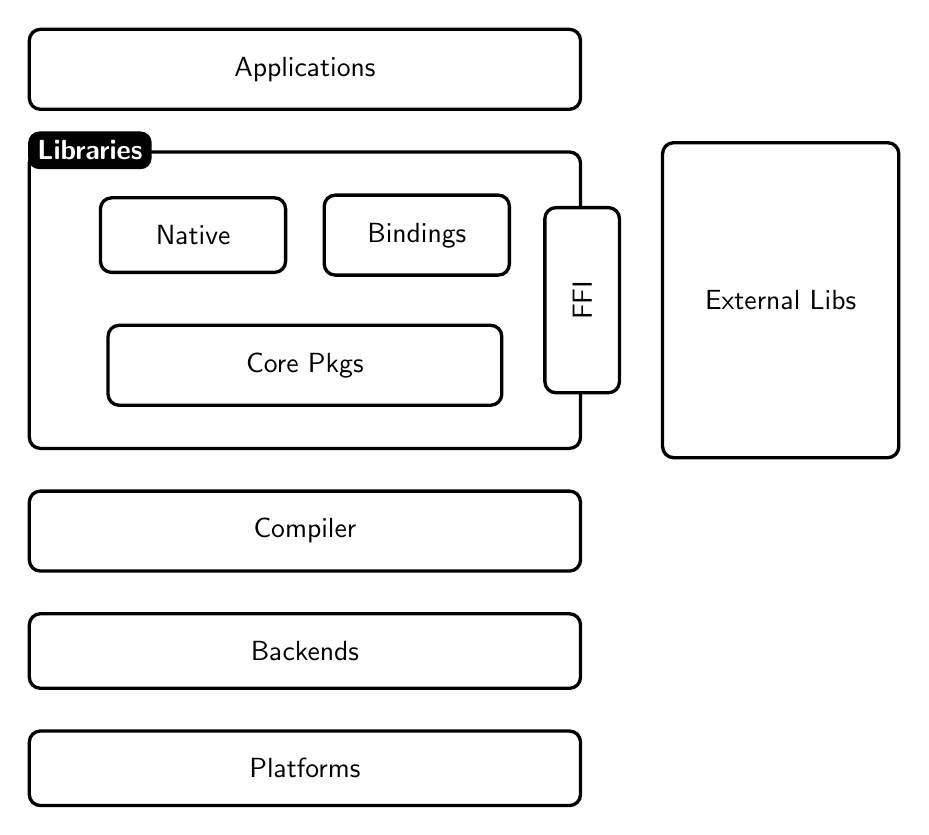
\begin{tikzpicture}[scale=1, shape aspect=1]

\node (center) at (0,0) {};

\node (stdlibs) [Box, WhiteBody,
                 left = 1mm of center] {Native};

\node (bindings) [Box, WhiteBody,
                  right = 1mm of center] {Bindings};

\node (core) [Box, WhiteBody,
              below = of center,
              minimum width = 50mm] {Core Pkgs};

\begin{pgfonlayer}{background layer}

\node (libs) [BorderBox, WhiteBody,
              fit=(stdlibs) (bindings) (core),
              minimum width = 70mm] {};
\node [BlackTitle, right] at (libs.north west) {Libraries};

\end{pgfonlayer}

\node (ffi) [Box, WhiteBody, rotate = 90] at (libs.east) {FFI};
\node (extlibs) [Box, WhiteBody,
                 right = of libs.east,
                 minimum width = 30mm,
                 minimum height = 40mm] {External Libs};

%% ---------------------------------------------------------------- [ Compiler ]
\node (compiler) [Box, WhiteBody, minimum width = 70mm,
                  below = 5mm of libs] {Compiler};
\node (backends) [Box, WhiteBody, minimum width = 70mm,
                  below = 5mm of compiler] {Backends};
\node (patflorm) [Box, WhiteBody, minimum width = 70mm,
                  below = 5mm of backends] {Platforms};

%% ------------------------------------------------------------ [ Applications ]
\node (apps) [Box, WhiteBody, minimum width = 70mm,
              above = 5mm of libs] {Applications};
\end{tikzpicture}
\end{document}
